\documentclass[11pt,compress,t,notes=noshow, xcolor=table]{beamer}
\usepackage[]{graphicx}\usepackage[]{color}
% maxwidth is the original width if it is less than linewidth
% otherwise use linewidth (to make sure the graphics do not exceed the margin)
\makeatletter
\def\maxwidth{ %
  \ifdim\Gin@nat@width>\linewidth
    \linewidth
  \else
    \Gin@nat@width
  \fi
}
\makeatother

\definecolor{fgcolor}{rgb}{0.345, 0.345, 0.345}
\newcommand{\hlnum}[1]{\textcolor[rgb]{0.686,0.059,0.569}{#1}}%
\newcommand{\hlstr}[1]{\textcolor[rgb]{0.192,0.494,0.8}{#1}}%
\newcommand{\hlcom}[1]{\textcolor[rgb]{0.678,0.584,0.686}{\textit{#1}}}%
\newcommand{\hlopt}[1]{\textcolor[rgb]{0,0,0}{#1}}%
\newcommand{\hlstd}[1]{\textcolor[rgb]{0.345,0.345,0.345}{#1}}%
\newcommand{\hlkwa}[1]{\textcolor[rgb]{0.161,0.373,0.58}{\textbf{#1}}}%
\newcommand{\hlkwb}[1]{\textcolor[rgb]{0.69,0.353,0.396}{#1}}%
\newcommand{\hlkwc}[1]{\textcolor[rgb]{0.333,0.667,0.333}{#1}}%
\newcommand{\hlkwd}[1]{\textcolor[rgb]{0.737,0.353,0.396}{\textbf{#1}}}%
\let\hlipl\hlkwb

\usepackage{framed}
\makeatletter
\newenvironment{kframe}{%
 \def\at@end@of@kframe{}%
 \ifinner\ifhmode%
  \def\at@end@of@kframe{\end{minipage}}%
  \begin{minipage}{\columnwidth}%
 \fi\fi%
 \def\FrameCommand##1{\hskip\@totalleftmargin \hskip-\fboxsep
 \colorbox{shadecolor}{##1}\hskip-\fboxsep
     % There is no \\@totalrightmargin, so:
     \hskip-\linewidth \hskip-\@totalleftmargin \hskip\columnwidth}%
 \MakeFramed {\advance\hsize-\width
   \@totalleftmargin\z@ \linewidth\hsize
   \@setminipage}}%
 {\par\unskip\endMakeFramed%
 \at@end@of@kframe}
\makeatother

\definecolor{shadecolor}{rgb}{.97, .97, .97}
\definecolor{messagecolor}{rgb}{0, 0, 0}
\definecolor{warningcolor}{rgb}{1, 0, 1}
\definecolor{errorcolor}{rgb}{1, 0, 0}
\newenvironment{knitrout}{}{} % an empty environment to be redefined in TeX

\usepackage{alltt}
\newcommand{\SweaveOpts}[1]{}  % do not interfere with LaTeX
\newcommand{\SweaveInput}[1]{} % because they are not real TeX commands
\newcommand{\Sexpr}[1]{}       % will only be parsed by R
\newcommand{\xmark}{\ding{55}}%


\usepackage[english]{babel}
\usepackage[utf8]{inputenc}

\usepackage{dsfont}
\usepackage{verbatim}
\usepackage{amsmath}
\usepackage{amsfonts}
\usepackage{amssymb}
\usepackage{bm}
\usepackage{csquotes}
\usepackage{multirow}
\usepackage{longtable}
\usepackage{booktabs}
\usepackage{enumerate}
\usepackage[absolute,overlay]{textpos}
\usepackage{psfrag}
\usepackage{algorithm}
\usepackage{algpseudocode}
\usepackage{eqnarray}
\usepackage{arydshln}
\usepackage{tabularx}
\usepackage{placeins}
\usepackage{tikz}
\usepackage{setspace}
\usepackage{colortbl}
\usepackage{mathtools}
\usepackage{wrapfig}
\usepackage{bm}
\usepackage{amsmath}
\usepackage{pifont}
\usepackage{xcolor} %colored math symbols

\usetikzlibrary{shapes,arrows,automata,positioning,calc,chains,trees, shadows}
\tikzset{
  %Define standard arrow tip
  >=stealth',
  %Define style for boxes
  punkt/.style={
    rectangle,
    rounded corners,
    draw=black, very thick,
    text width=6.5em,
    minimum height=2em,
    text centered},
  % Define arrow style
  pil/.style={
    ->,
    thick,
    shorten <=2pt,
    shorten >=2pt,}
}

\usepackage{subfig}

% Defines macros and environments
\usepackage{../../style/lmu-lecture}


\let\code=\texttt
\let\proglang=\textsf

\setkeys{Gin}{width=0.9\textwidth}

\setbeamertemplate{frametitle}{\expandafter\uppercase\expandafter\insertframetitle}

\usepackage{bbm}
% basic latex stuff
\newcommand{\pkg}[1]{{\fontseries{b}\selectfont #1}} %fontstyle for R packages
\newcommand{\lz}{\vspace{0.5cm}} %vertical space
\newcommand{\dlz}{\vspace{1cm}} %double vertical space
\newcommand{\oneliner}[1] % Oneliner for important statements
{\begin{block}{}\begin{center}\begin{Large}#1\end{Large}\end{center}\end{block}}


%new environments
\newenvironment{vbframe}  %frame with breaks and verbatim
{
 \begin{frame}[containsverbatim,allowframebreaks]
}
{
\end{frame}
}

\newenvironment{vframe}  %frame with verbatim without breaks (to avoid numbering one slided frames)
{
 \begin{frame}[containsverbatim]
}
{
\end{frame}
}

\newenvironment{blocki}[1]   % itemize block
{
 \begin{block}{#1}\begin{itemize}
}
{
\end{itemize}\end{block}
}

\newenvironment{fragileframe}[2]{  %fragile frame with framebreaks
\begin{frame}[allowframebreaks, fragile, environment = fragileframe]
\frametitle{#1}
#2}
{\end{frame}}


\newcommand{\myframe}[2]{  %short for frame with framebreaks
\begin{frame}[allowframebreaks]
\frametitle{#1}
#2
\end{frame}}

\newcommand{\remark}[1]{
  \textbf{Remark:} #1
}


\newenvironment{deleteframe}
{
\begingroup
\usebackgroundtemplate{
\includegraphics[width=\paperwidth,height=\paperheight]{../style/color/red.png}}
 \begin{frame}
}
{
\end{frame}
\endgroup
}
\newenvironment{simplifyframe}
{
\begingroup
\usebackgroundtemplate{
\includegraphics[width=\paperwidth,height=\paperheight]{../style/color/yellow.png}}
 \begin{frame}
}
{
\end{frame}
\endgroup
}\newenvironment{draftframe}
{
\begingroup
\usebackgroundtemplate{
\includegraphics[width=\paperwidth,height=\paperheight]{../style/color/green.jpg}}
 \begin{frame}
}
{
\end{frame}
\endgroup
}
% https://tex.stackexchange.com/a/261480: textcolor that works in mathmode
\makeatletter
\renewcommand*{\@textcolor}[3]{%
  \protect\leavevmode
  \begingroup
    \color#1{#2}#3%
  \endgroup
}
\makeatother


\input{../../latex-math/basic-math}
\input{../../latex-math/basic-ml}
\input{../../latex-math/ml-nn}


\newcommand{\titlefigure}{figure/xor1.png}
\newcommand{\learninggoals}{
  \item Example problem a single neuron can not solve but a single hidden layer net can
}

\title{Deep Learning}
\date{}

\begin{document}


\lecturechapter{XOR-Problem}
\lecture{I2DL}

\begin{vbframe}{Example: XOR Problem}
  \begin{itemize}
    \item Suppose we have four data points $$X = \{(0,0)^\top, (0,1)^\top, (1,0)^\top, (1,1)^\top \}$$
    \item The XOR gate (exclusive or) returns true, when an odd number of inputs are true:
  \end{itemize}
  \begin{table}
    \centering
      \begin{tabular}{ccc}
        \textbf{$x_1$}  & \textbf{$x_2$}  & \textbf{XOR} $= y$ \\
        \hline
        \hline
        $0$             &   $0$           &  $0$ \\
        $0$             &   $1$           &  $1$ \\
        $1$             &   $0$           &  $1$ \\
        $1$             &   $1$           &  $0$
      \end{tabular}
  \end{table}
  \begin{itemize}
    \item Can you learn the target function with a logistic regression model? \\
    % (Aside from statistical generalization, we just want to learn the training data!)
  \end{itemize}
\framebreak
  \begin{minipage}{0.45\textwidth}
    \begin{itemize}
      \item Logistic regression can not solve this problem. %and will always output $0.5$. \\
      In fact, any model using simple hyperplanes for separation can not (including a single neuron).
      \lz
      \item A small neural net can easily solve the problem by transforming the space!
    \end{itemize}
  \end{minipage}
  \begin{minipage}{0.5\textwidth}
    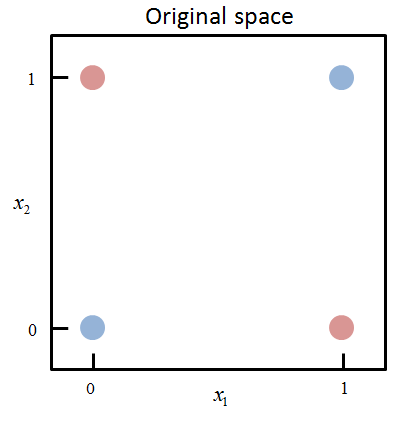
\includegraphics{figure/xor1.png}%
  \end{minipage}\hfill
\framebreak
  \begin{itemize}
    \item Consider the following model:
  \end{itemize}
    \begin{figure}
      \centering
        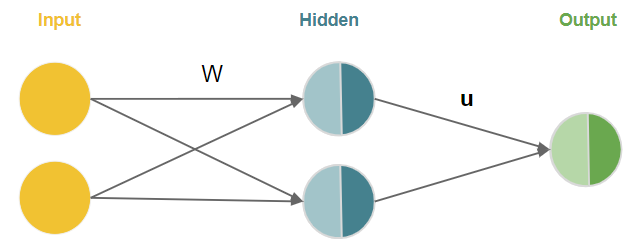
\includegraphics[width=8cm]{figure/xor_rep.png}%
        \caption{A neural network with two neurons in the hidden layer. The matrix $\Wmat$ describes the mapping from $\xv$ to $\hidz$. The vector $\wtu$ from $\hidz$ to $y$.}
    \end{figure}
\framebreak
  \begin{itemize}
    \item Let use ReLU $\sigma(z) = \max\left\{0, z \right\}$ as activation function and a simple thresholding function $\tau(z) = [ z > 0 ] =  \begin{cases} 1 & \text{ if } z > 0 \\ 0 & \text{otherwise} \end{cases} $ \\ as output transformation function. We can represent the architecture of the model by the following equation: 
  \end{itemize}
  \begin{eqnarray*}
    f(\xv~|~\thetah) &=& f(\xv~|~ \Wmat, \biasb, \wtu, \biasc) = \tau\left(\wtu^\top\sigma(\Wmat^\top \xv+\biasb)+\biasc\right) \\
                &=& \tau\left(\wtu^\top \max\{0, \Wmat^\top \xv+\biasb\} + \biasc\right)
  \end{eqnarray*}
  % \begin{footnotesize}
  % \textbf{Note:} To simplify calculations, we \enquote{falsely} treat the problem as a regression problem (no final output transformation $\tau$ to map scores to $[0, 1]$). We will see later that transformation to $[0, 1]$ is not necessary in this very special case.
  % \end{footnotesize}
  \begin{itemize}
    \item So how many parameters does our model have?
    \begin{itemize}
      \item In a fully connected neural net, the number of connections between the nodes equals our parameters: $$\underbrace{(2 \times 2)}_{W} + \underbrace{(2 \times 1)}_{\biasb} + \underbrace{(2 \times 1)}_{\wtu} + \underbrace{(1)}_{c} = 9$$
    \end{itemize}
  \end{itemize}
\framebreak
  \begin{eqnarray*}
   \text{Let} \ \Wmat = \begin{pmatrix}
      1 & 1 \\
      1 & 1
    \end{pmatrix}, \
      \biasb = \begin{pmatrix}
      0 \\
      -1
    \end{pmatrix}, \
      \wtu = \begin{pmatrix}
      1 \\
      -2
    \end{pmatrix}, \
      c = - 0.5
  \end{eqnarray*}
  \begin{eqnarray*}
    \Xmat = \begin{pmatrix}
      0 & 0 \\
      0 & 1 \\
      1 & 0 \\
      1 & 1
    \end{pmatrix}, \
    \Xmat \Wmat = \begin{pmatrix}
      0 & 0 \\
      1 & 1 \\
      1 & 1 \\
      2 & 2
    \end{pmatrix}, \
      \Xmat \Wmat + \bm{B} = \begin{pmatrix}
        0 & -1 \\
        1 & 0 \\
        1 & 0 \\
        2 & 1
    \end{pmatrix}
  \end{eqnarray*}
%\vspace{4mm}
 \footnotesize{Note: $\Xmat$ is a $(n \times p)$ design matrix in which the \textit{rows} correspond to the data points. $\Wmat$, as usual, is a $(p \times m)$ matrix where each \textit{column} corresponds to a single (hidden) neuron. $\bm{B}$ is a ($n \times m$) matrix with $\biasb$ duplicated along the rows.}
 \begin{figure}
    \centering
      \scalebox{0.6}{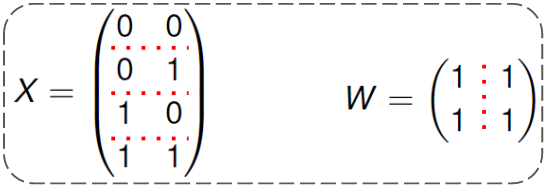
\includegraphics{figure/rowcol.png}}
  \end{figure}
 \framebreak
 \normalsize{
 \begin{eqnarray*}
   \text{Let} \ \Wmat = \begin{pmatrix}
      1 & 1 \\
      1 & 1
    \end{pmatrix}, \
      \biasb = \begin{pmatrix}
      0 \\
      -1
    \end{pmatrix}, \
      \wtu = \begin{pmatrix}
      1 \\
      -2
    \end{pmatrix}, \
      c = - 0.5
  \end{eqnarray*}
  \begin{eqnarray*}
  \Xmat = \begin{pmatrix}
      0 & 0 \\
      0 & 1 \\
      1 & 0 \\
      1 & 1
    \end{pmatrix}, \
    \Xmat\Wmat = \begin{pmatrix}
      0 & 0 \\
      1 & 1 \\
      1 & 1 \\
      2 & 2
    \end{pmatrix}, \
      \Xmat \Wmat + \bm{B} = \begin{pmatrix}
        0 & -1 \\
        1 & 0 \\
        1 & 0 \\
        2 & 1
    \end{pmatrix}
  \end{eqnarray*}
  \begin{eqnarray*}
    \bm{Z} = \max\{0, \Xmat \Wmat+\bm{B}\}
    &=&
    \begin{pmatrix}
      0 & 0 \\
      1 & 0 \\
      1 & 0 \\
      2 & 1
    \end{pmatrix}
  \end{eqnarray*}
  \begin{itemize}
    \item Note that we computed all examples at once.
  \end{itemize}

\framebreak
  \begin{minipage}{0.45\textwidth}
    \begin{itemize}
      \item The input points are mapped into transformed space to
        \begin{eqnarray*}
          \bm{Z} = \begin{pmatrix}
              0 & 0 \\
              1 & 0 \\
              1 & 0 \\
              2 & 1
          \end{pmatrix}
        \end{eqnarray*}
    %  \item[] which is easily separable.
    \end{itemize}
  \end{minipage}
  \begin{minipage}{0.5\textwidth}
    \includegraphics<1>{figure/xor2_2.png}%
  \end{minipage}\hfill
  
\framebreak
  \begin{minipage}{0.45\textwidth}
    \begin{itemize}
      \item The input points are mapped into transformed space to
        \begin{eqnarray*}
          \bm{Z} = \begin{pmatrix}
              0 & 0 \\
              1 & 0 \\
              1 & 0 \\
              2 & 1
          \end{pmatrix}
        \end{eqnarray*}
      \item[] which is easily separable.
    \end{itemize}
  \end{minipage}
  \begin{minipage}{0.5\textwidth}
    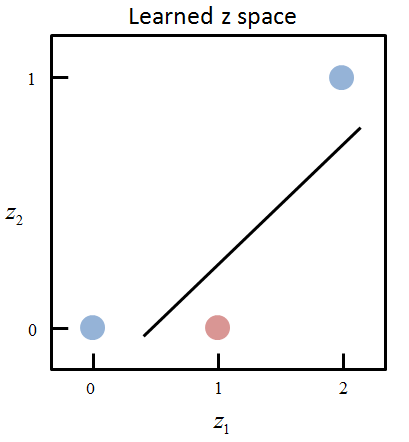
\includegraphics{figure/xor2.png}%
  \end{minipage}\hfill
  
\framebreak
  \begin{itemize}
    \item In a final step we have to multiply the activated values of matrix $\bm{Z}$ with the vector $\wtu$ and add the bias term $c$:
  \end{itemize}
  \begin{eqnarray*}
    f(\xv ~|~ \Wmat, \biasb, \wtu, c) &=&
    \begin{pmatrix}
      0 & 0 \\
      1 & 0 \\
      1 & 0 \\
      2 & 1
    \end{pmatrix}
    \begin{pmatrix}
      1 \\
      -2
    \end{pmatrix} + 
    \begin{pmatrix}
      - 0.5 \\
      - 0.5 \\
      - 0.5 \\
      - 0.5
    \end{pmatrix}
    =
    \begin{pmatrix}
      - 0.5 \\
      0.5 \\
      0.5 \\
      - 0.5
    \end{pmatrix}
  \end{eqnarray*}
  \begin{itemize}
    \item And then apply the step function $\tau(z) = [z > 0 ]$.  This solves the XOR problem perfectly!
  \end{itemize}
  \begin{table}
    \centering
      \begin{tabular}{ccc}
        \textbf{$x_1$}  & \textbf{$x_2$}  & \textbf{XOR} = y\\
        \hline
        \hline
        $0$             &   $0$           &  $0$ \\
        $0$             &   $1$           &  $1$ \\
        $1$             &   $0$           &  $1$ \\
        $1$             &   $1$           &  $0$
      \end{tabular}
  \end{table}
  }
\end{vbframe}



\begin{frame} {Neural Networks : Optimization}
  \begin{itemize}
    \item In this simple example we actually \enquote{guessed} the values of the parameters for $\textbf{W}$, $\biasb$, $\wtu$ and $c$.
    \vspace{3mm}
    \item That won't work for more sophisticated problems!
    \vspace{3mm}
    %\item To learn the right weights (and biases), we once again have to rely on iterative algorithms like gradient descent.
    \item We will learn later about iterative optimization algorithms for automatically adapting weights and biases.
    \vspace{3mm}
    \item An added complication is that the loss function is no longer convex. Therefore, there might not exist a single minimum. 
    %Therefore, gradient descent can only find a local minimum. 
 %   \vspace{3mm}
  %  \item An extremely efficient method to compute gradients called backpropogation will be covered in the next lecture.
  \end{itemize}
\end{frame}

\endlecture
\end{document}